\documentclass[1p]{afparticle}
\usepackage{lipsum}
\begin{document}
%%%%%%%%%%%%%%%%%%%%%%%%%%%%%%%%%%%%%%%%%%%%%%%%%%%%%%%%%%%%%%%
% Information about the current issue
%%%%%%%%%%%%%%%%%%%%%%%%%%%%%%%%%%%%%%%%%%%%%%%%%%%%%%%%%%%%%%%
% Volume
\volumenumber{2}
% Issue
\issuenumber{1}
% Year
\publicationyear{2014}
% Number of the paper in the journal
\papernumber{2}
% First page
\startpage{256}
%%%%%%%%%%%%%%%%%%%%%%%%%%%%%%%%%%%%%%%%%%%%%%%%%%%%%%%%%%%%%%%%
% Information about the paper
%%%%%%%%%%%%%%%%%%%%%%%%%%%%%%%%%%%%%%%%%%%%%%%%%%%%%%%%%%%%%%%
% Title.  If necessary, put the short title in the [..]
\title[Research Title]{Unnecessarily Complicated Research Title}
% Authors.  The star denotes thecorressponding author
\author*{John Smith}
\address{Department, University, City, State, Country, Phone, E-mail}
\author{Tom F. Johnson}
\address{Department, University, City, State, Country}
\author{Peter Sellers}
\address{Department, University, City, State, Country}
\author{Jay P. Singh}
\address{Department, University, City, State, Country}
% If necessary, redefine \shortauthors
\renewcommand\shortauthors{John Smith et al}
% Abstract
\begin{abstract}
  \lipsum[1]
\end{abstract}
% Keywords
\begin{keyword}
  One\sep Two\sep Three
\end{keyword}

% Technical information
% Reception
\received{April 1, 2013}
% Revision;  can be repeated
\revised{May 20, 2013}
\revised{June 15, 2013}
% Acceptance
\accepted{July 30, 2013}

% Making title
\maketitle

\section{First section}
\lipsum[2]

% In-text citation
As shown by \citet{Haidt07}, people are selfish, but morally
motivated.  See also the work by
\citet{Stapel08042011}. 

% Parenthetical citations
The method in \citep{Zintzaras10} may help.

\subsection{A subsection}

\lipsum[4]

\subsubsection{A subsubsection}

%%%%%%%%%%%%%%%%%%%%%%%%%%%%%%%%%%%%%%%%%%%%%%%%%%%%%%%%%%%%
%
%  TABLE
%
% Put caption before the table.  Use booktabs for table
% formatting 
%%%%%%%%%%%%%%%%%%%%%%%%%%%%%%%%%%%%%%%%%%%%%%%%%%%%%%%%%%%%%
\begin{table}
  \centering
  \caption{A sample table}
  \label{tab:sample}
  \begin{tabular}{lrrr}
    \toprule
    Item & Units & Cost per unit, \$ & Total cost, \$\\
    \midrule
    Stuffed Gnus &  5  & 12.50  & 62.50 \\
    Memory Sticks & 4  &  6.00  & 24.00\\
    \midrule
    Total & & & 86.50\\
    \bottomrule
  \end{tabular}
\end{table}


%%%%%%%%%%%%%%%%%%%%%%%%%%%%%%%%%%%%%%%%%%%%%%%%%%%%%%%%%%%%
%
%  FIGURE
%
%%%%%%%%%%%%%%%%%%%%%%%%%%%%%%%%%%%%%%%%%%%%%%%%%%%%%%%%%%%%%
\begin{figure}
  \centering
  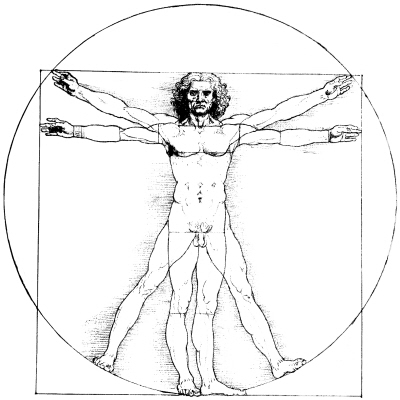
\includegraphics{vitruvian}
  \caption{A sample figure}
  \label{fig:sample}
\end{figure}

\lipsum[7-21]


% Bibliography
\bibliography{afpsample}
\bibliographystyle{apacite}

% This should be the last command
\printbackmatter

\end{document}
